%!TEX program = xelatex
\documentclass{progartcn}
\usepackage{graphicx}
\usepackage[dvipsnames]{xcolor}
\usepackage{wrapfig}
\usepackage{enumerate}
\usepackage{appendix}
\usepackage{amsmath,mathrsfs,amsfonts}
\usepackage{booktabs}
\usepackage{tabularx}
\usepackage{colortbl}
\usepackage{multirow,makecell}
\usepackage{multicol}
\usepackage{ulem} % \uline
\usepackage{listings}
\usepackage{tikz}
\usepackage{tcolorbox}
\usepackage{fontawesome}
\usepackage{float}   %{H}
\usepackage{multicol}%分栏 %\begin{multicols}{2} %\end{multicols}
\usepackage{arydshln}
\setcounter{secnumdepth}{4}		%增加编号深度
\setcounter{tocdepth}{3}		%增加目录深度
\usepackage{hyperref}     %生成pdf书签
\hypersetup{hidelinks,
	colorlinks=true,
	allcolors=black,
	pdfstartview=Fit,
	breaklinks=true
}       %去掉目录的红色框框
\pagestyle{plain}%设置页码
\usepackage{fontspec}
\usepackage{enumitem} %调整有序列表的行距
\usepackage{makecell}
\setCJKfamilyfont{hwzs}{STZHONGS.TTF}
\newcommand{\hwzs}{\CJKfamily{hwzs}}
\begin{document}

\sloppy % 解决中英文混排文字超出边界问题

\newpage

\thispagestyle{empty}
\begin{center}	
%	\parbox[t][1cm][c]{\textwidth}{\large
%		\begin{center} {\textbf{美团商业分析精英大赛}}\end{center} }
		
\includegraphics[width=2in]{2.jpg}\\
	\parbox[t][4cm][c]{\textwidth}{\Huge
		\begin{center} {\heiti\textbf{西南大学\\人工智能学院智能科学大类}}\end{center} }
		
	\parbox[t][1cm][t]{\textwidth}{
		\begin{center}  \end{center} }
	
	\parbox[t][1cm][c]{\textwidth}{\huge
		\begin{center} {\hwzs{《程序设计综合课程设计》报告}}\end{center} }
	\parbox[t][12cm][b]{\textwidth}{
		\begin{center}
			\Large{
			\begin{tabular}{rl}
				% after \\: \hline or \cline{col1-col2} \cline{col3-col4} ...
				\textbf{题\;\;\;\;\;\;\;目}:& \underline{QQ好友管理系统软件开发设计\;} \\
				\textbf{级、专业}:& \underline{2020 级 智能科学与技术   专业   6   班} \\
				\textbf{学生学号}:& \underline{\;\;\;\;\;\;\;\;\;\;\;\;222020335220177\;\;\;\;\;\;\;\;\;\;\;\;}\\
				\textbf{学生姓名}:& \underline{\;\;\;\;\;\;\;\;\;\;\;\;\;\;\;\;\;\;\;严中圣\;\;\;\;\;\;\;\;\;\;\;\;\;\;\;\;\;\;\;\;}\\
				\textbf{指导教师}:& \underline{\;\;\;\;\;\;\;\;\;\;\;\;\;\;\;\;\;\;\;\;\;\;\;\;\;\;\;\;\;\;\;\;\;\;\;\;\;\;\;\;\;\;\;\;\;\;\;\;\;\;}\\
				\textbf{提交日期}:& \underline{\;\;\;\;\;\;\;\;\;\;\;\;2021  年  7  月  10 日\;\;\;\;\;\;\;\;\;\;\;\;}
			\end{tabular}}
		\end{center} }
	
%	\parbox[t][2cm][b]{\textwidth}{
%		\begin{center} {\large\textbf{\textsf \today}} \end{center} }
\end{center}


\clearpage
%=============================================================================================
%\maketitle
\thispagestyle{empty}
\tableofcontents  %目录
\newpage


\section{实践课程设计任务描述}
\subsection{实践课程设计目的}
本次程序设计实践课程设计要求运用所学编程技能独立开发一个小型应用软件,目的在于锻炼自身的编程技能以及提高对于软件架构设计的理解、应用;其次能够简单掌握数据库的设计及软件界面设计等操作,熟悉软件开发从设计到架构到封装打包的过程,对于计算机学科专业学生来说无疑是一次极佳的实践机会。

\subsection{实践课程设计要求}

本次选题为模拟QQ实现好友管理系统,具体设计要求如下:
\begin{enumerate}[itemsep=0.01pt]
	\item[(1)] 能够实现QQ登录系统并具有独立的登录界面;
	\item[(2)] 能够实现用户通过口令登录,且密码采用MD5加密算法封装验证;
	\item[(3)] 能够实现QQ好友管理系统并具有独立的系统界面;
	\item[(4)] 能够实现通过鼠标触发事件进行软件操作;
	\item[(5)] 能够自主设计数据库作为数据存储环境;
	\item[(6)] 能够增加好友(默认对方已经同意请求)、删除好友、移动好友分组、查看好友详细信息等;
	\item[(7)] 能够实现好友分组以及分组的增删、修改等;
	\item[(8)] 能够修改好友列表中已有好友信息(如备注等);
	\item[(9)] 能够按照首字母或分组查找好友;
	\item[(10)] 能够将好友加入黑名单,加入黑名单的好友不能再被查找,并设置黑名单人数上限。
\end{enumerate}

\subsection{实践课程设计背景}

在互联网极为发达的今天,网络通信已经成为人们生活中不可或缺的部分,而每个成熟的聊天软件都需要一个完善的好友管理系统作为支撑。本次实践通过模拟开发QQ聊天软件,旨在对常见操作背后原理进行熟悉并实践开发,为以后的工程设计实践奠定实践经验。

\subsection{实践课程设计作品用途}

本次设计开发的模拟QQ软件,现有基础可支持聊天软件的基础操作,后续在配合上TCP网络传输协议与聊天室界面设计以后即可实现正常的网络通信,如再配合服务器的开发,即可实现多人聊天室的信息传输以及多用户的聊天平台搭建。

\section{功能需求分析}

\subsection{后台数据库搭建环境配置}

对于本次设计的好友管理系统,必须依赖后台的MySQL数据库进行数据存储,否则则无法形成一个完整的管理系统,故在正式进入开发前先要对项目工程进行数据库设计及配置。本次项目开发基于QT Creator开发环境,我们首先对QT进行MySQL环境配置。

\begin{enumerate}[itemsep=0.01pt]
	\item[(1)] 首先在项目配置文件QQ$ \_ $model.pro中添加“QT+=SQL”配置项;同时在QT中安装MySQL驱动QMySQL;
	\item[(2)] 其次在头文件mainwindow.h中建立方法createMysqlConn(),设置好待连接数据库的数据库管理系统、主机名、接口、用户名、密码以及需要需要调用的数据库名,调用Qsqldatabase类函数实现数据库连接并设置好提示消息“数据库已连接”/“数据库连接失败”;
	\item[(3)] 在主程序main.cpp中导入头文件mainwindow.h最先进行方法createMysqlConn()调用并在一次连接失败后尝试二次连接。至此数据库连接配置已完成。
\end{enumerate}

\subsection{用户验证登录系统实现}

用户验证登录系统需要包括数据库用户信息调出验证、用户选择“登录”或“退出”按钮、登录成功或失败提示指令,登录功能实现在logindialog.h头文件及logindialog.cpp源文件中。
\begin{enumerate}[itemsep=0.01pt]
	\item[(1)] 向logindialog.h中导入MySQL相关库,包括QDialog、QsqlQuery、QCryptographicHash分别用于数据库的连接、查询及MD5加密算法,其次声明变量与方法;
	\item[(2)] 在logindialog.cpp中设置登录界面大小及窗口位置,其次设置数据库调用指令将存储的用户密码与用户输入密码进行验证比对,并设置提示指令弹窗;
	\item[(3)] 向main.cpp中导入头文件“logindialog.h”,初始启动程序main.cpp后,数据库首先成功连接之后初始化登录界面,调用logindialog.cpp中的LoginDialog()方法,验证通过后即显示初始化好友管理界面。
\end{enumerate}

\subsection{好友管理系统实现}
好友管理系统主体程序包括main.cpp、mainwindow.h和mainwindow.cpp.

\begin{enumerate}[itemsep=0.01pt]
	\item[(1)] main.app
它是整个系统的主启动文件,在连接数据库与用户登录验证通过后执行初始化好友管理系统界面,即显示Mainwindow主窗口。
\item[(2)]mainwindow.h
它是程序头文件,包含程序中用到的各个全局变量的定义、方法声明,同时在此文件中设置了数据库连接的静态方法。
\item[(3)]mainwindow.app
它是本程序的主体源文件,其中包含各方法功能的具体实现代码,其中框架如下:\\
initMainWindow():执行系统主窗体初始化\\
onTableSelectChange(int row):在用户选择不同好友信息时进行表单更新\\
showFriendPhoto():显示QQ头像\\
loadPreFriends():用来在对应分组下拉框加载好友列表\\
onPreNameComboBoxChange():在改选好友时联动进行好友列表信息更新\\
FriendsTableView$\_$3$\_$clicked(const QModelIndex $ \& $index):联动显示好友信息\\
preGroupComboBox$\_$currentIndexChanged(int index):根据分组对应加载好友列表\\
preNameComboBox$\_$currentIndexChanged(int index):选择好友时联动显示好友信息\\
on$\_$DeletePushButton$\_$clicked():进行删除好友操作\\
on$\_$newUploadPushButton$\_$clicked():进行上传头像操作\\
on$\_$NewPutinPushButton$\_$clicked():进行添加好友操作\\
on$\_$ChangePushButton$\_$clicked():进行修改好友信息操作\\
on$\_$SearchPushButton$\_$clicked():进行好友搜索操作\\
从以上代码框架可看到整个程序的运作机制,一目了然。
\end{enumerate}

\subsection{功能组成结构图}

\begin{figure}[H]
	\centering
	
\includegraphics[width=0.8\textwidth]{2.png}
	\caption{\centering  MySQL friends$ \_ $inf视图创建过程图}
\end{figure}

\section{软件总体设计}

\subsection{软件开发环境}
\begin{enumerate}[itemsep=0.01pt]
	\item[(1)]Qt Creator 4.11.0,Based on Qt 5.14.0 (GCC 5.3.1 20160406 (Red Hat 5.3.1-6), 64 bit)
\item[(2)]Mysql 8.0.25-0ubuntu0.20.04.01
\item[(3)]OS:Ubuntu20.04LTS
\item[(4)]Opencv4.5.2
\end{enumerate}

\subsection{数据库设计}

\subsubsection{创建数据库}

在Mysql中创建数据库,名称为QQ$ \_ $model,其中建立三个表,分别为Group(好友分组表)、friendsList(好友信息表),Member(用户信息表)。

\subsubsection{设计表}

\begin{enumerate}[itemsep=0.01pt]
\item[(1)]表结构设计

Group表设计见下表
\begin{figure}[H]
	\centering
	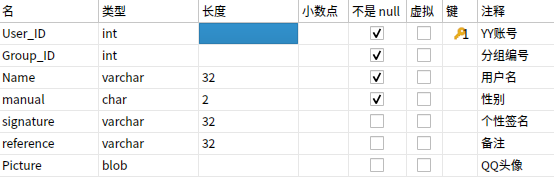
\includegraphics[width=0.7\textwidth]{10.png}
	\caption{\centering  Group表设计图示}
\end{figure}

friendsList表设计见下表
\begin{figure}[H]
	\centering
	
\includegraphics[width=0.7\textwidth]{11.png}
	\caption{\centering friendsList表设计图示}
\end{figure}

Member表设计见下表
\begin{figure}[H]
	\centering
	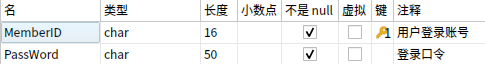
\includegraphics[width=0.7\textwidth]{12.png}
	\caption{\centering Member表设计图示}
\end{figure}

\item[(2)]外键关联

设计好表结构之后,为表之间建立外键连接。本项目在friendsList上建立一个外键关联,运用Navicat for MySQL数据库可视化工具进行设计,具体设计见下表:

\begin{figure}[H]
	\centering
	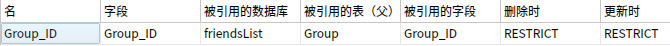
\includegraphics[width=0.8\textwidth]{13.png}
	\caption{\centering friendsList表外键关联信息表}
\end{figure}

\item[(3)]数据录入

设计好表及其关联之后,向各表中预先录入一些数据记录以供后面测试运行程序之用,具体见下列表:

\begin{figure}[H]
	\centering
	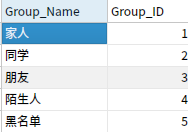
\includegraphics[width=0.25\textwidth]{14.png}
	\caption{\centering Group表预先录入信息}
\end{figure}

\begin{figure}[H]
	\centering
	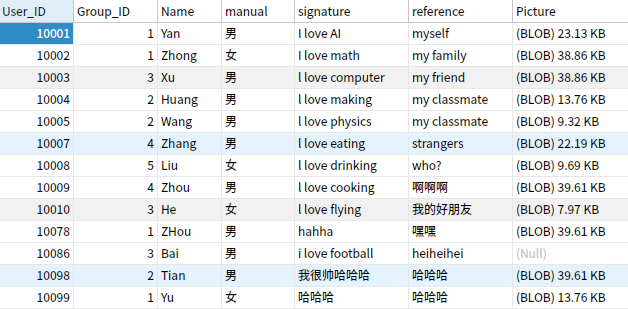
\includegraphics[width=0.8\textwidth]{15.png}
	\caption{\centering friendsList表预先录入信息}
\end{figure}

\begin{figure}[H]
	\centering
	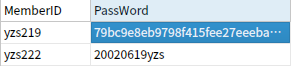
\includegraphics[width=0.5\textwidth]{16.png}
	\caption{\centering Member表预先录入信息}
\end{figure}

此外,对于图片的录入,我们通过编写代码将其通过二进制编码录入,具体代码如下:

\begin{lstlisting}[language=c++]
QString photoPath="/home/god/QQ_model/QQ_photos/10.jpeg"; //储存路径
QFile photoFile(photoPath);
if (photoFile.exists())
{	//存入数据库
	QByteArray picdata;
	photoFile.open(QIODevice::ReadOnly);  //只读模式加载图片
	picdata=photoFile.readAll();
	photoFile.close();
	QVariant var(picdata);
	QString sqlstr = "update FriendsList set Picture =? where User_ID=10010";  //编写数据库更新命令
	query.prepare(sqlstr);
	query.addBindValue(var);
}
if (!query.exec())
{
	QMessageBox::information(0,QObject::tr("提示"),"照片写入失败!");
}
else
{
	QMessageBox::information(0,QObject::tr("提示"),"照片上传成功!");
}

\end{lstlisting}
\end{enumerate}

\subsubsection{创建视图}

根据应用需要,本项目需要建立一个视图friends$ \_ $inf,用于显示好友的基本信息,创建如下图

\begin{figure}[H]
	\centering
	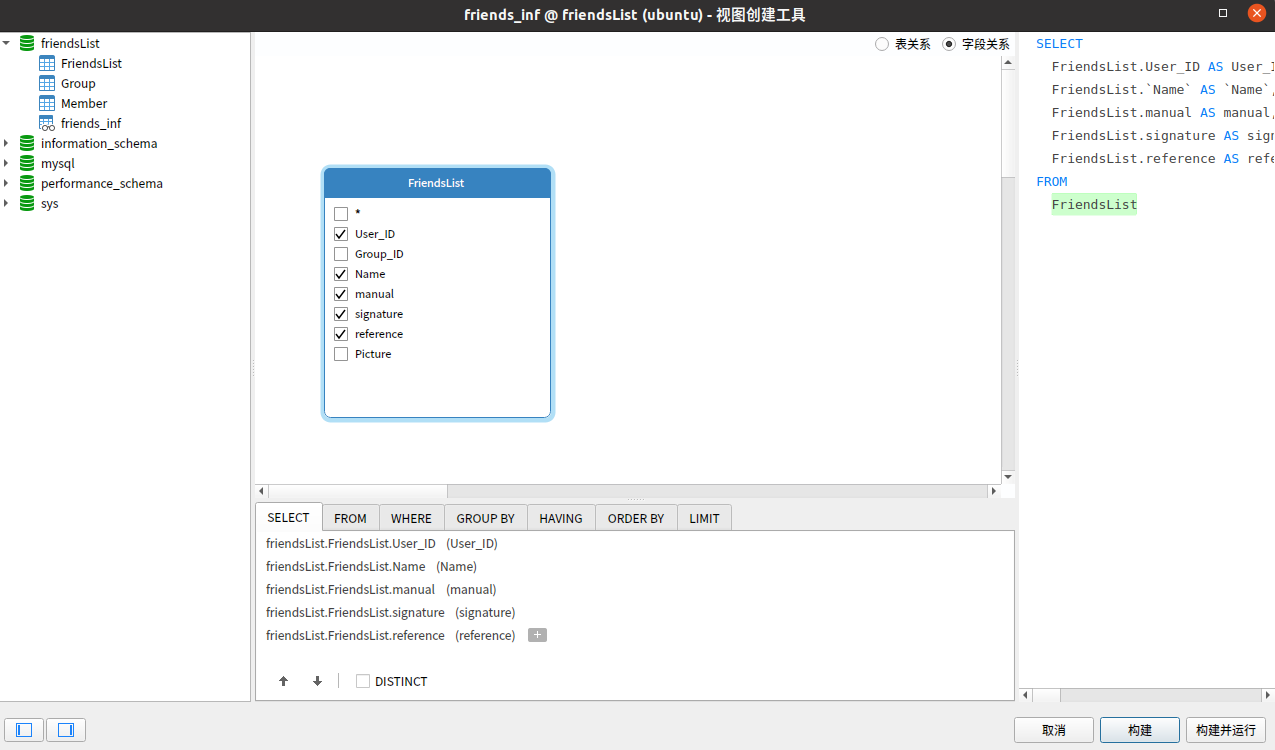
\includegraphics[width=0.8\textwidth]{4.png}
	\caption{\centering  MySQL friends$ \_ $inf视图创建过程图}
\end{figure}
有了这个视图,就可以在程序中通过模型载入好友的基本信息显示于界面上,而屏蔽掉无关的信息项,非常方便。
这样,系统运行所依赖的后台数据库就全部建立起来。

\subsection{界面设计}

\subsubsection{总体设计}

我们利用QT Creator的界面设计控件QT designer进行UI设计,为了使好友管理系统界面功能更加集中统一,我们将QT的stacked Widget控件与Tool Box控件结合使用,在一个统一的“好友管理”框中沿纵向布置“添加好友”、“删除好友”和“好友信息”页,分别对应系统功能需求中这三大模块,设计效果图见下图:

\begin{figure}[H]
	\centering
	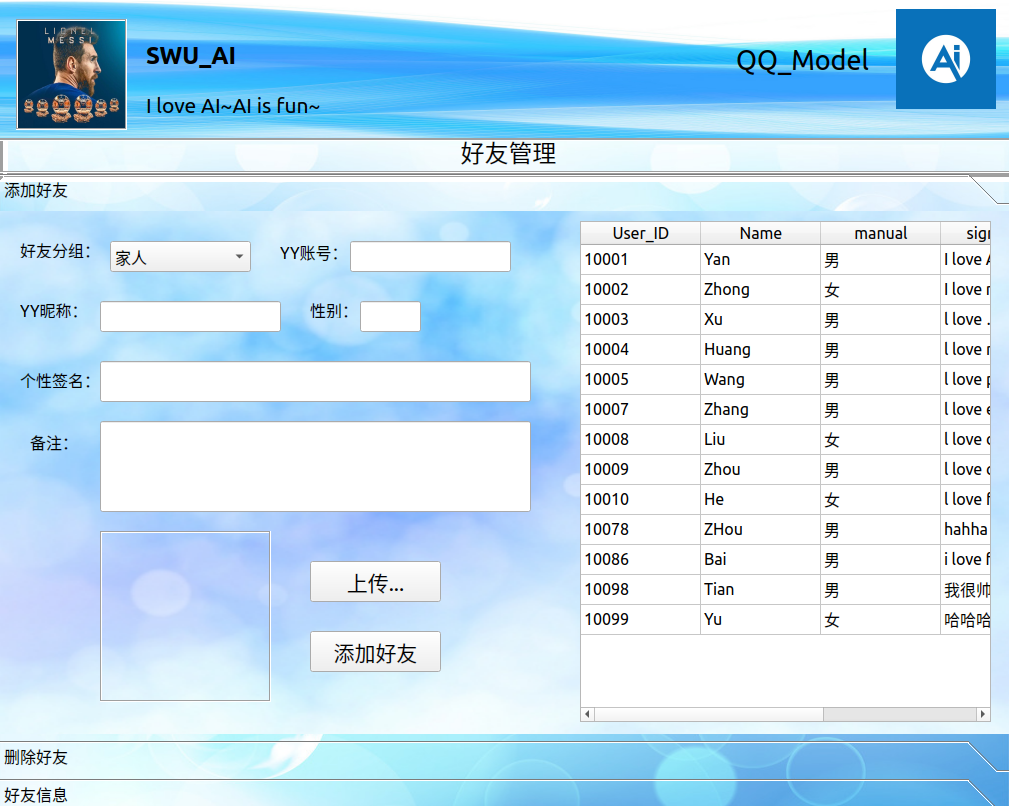
\includegraphics[width=0.5\textwidth]{5.png}
	\caption{\centering  初始化主窗体页面效果图}
\end{figure}

\subsubsection{"添加好友"页}

“添加好友”页界面设计效果如下图所示,界面各控件属性设置见下表

\begin{figure}[H]
	\centering
	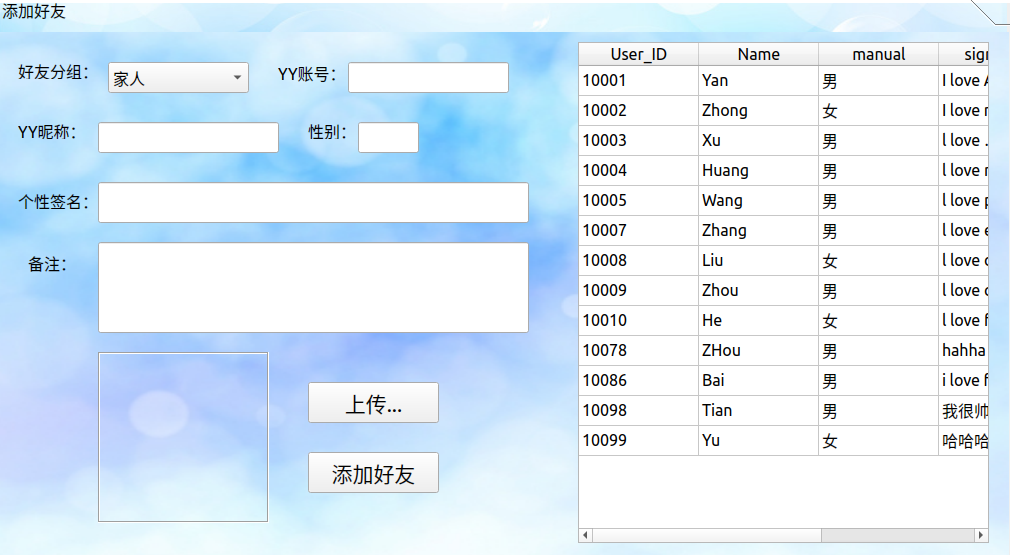
\includegraphics[width=0.6\textwidth]{6.png}
	\caption{\centering  “添加好友”页面效果图}
\end{figure}

\begin{table}[H]
	\renewcommand{\arraystretch}{1.0}
	\centering
	\caption{\centering “添加好友”页界面各控件属性设置}
	\begin{tabular}{lll}
		\toprule[1.5pt]
	名称                   & 类型          & 属性设置                                                                                                                                                                  \\
		\midrule[1pt]
		newGroupComboBox     & QComboBox   & 默认                                                                                                                                                                    \\
		newIDLineEdit        & QLineEdit   & 默认                                                                                                                                                                    \\
		newNameLineEdit      & QLineEdit   & 默认                                                                                                                                                                    \\
		newmanualLineEdit    & QLineEdit   & 默认                                                                                                                                                                    \\
		newSignatureLineEDit & QLineEdit   & 默认                                                                                                                                                                    \\
		newReferenceLineEdit & QLineEdit   & 默认                                                                                                                                                                    \\
		newPictureLabel      & QLabel      & \makecell[l]{frameshape:Box\\ frameShadow:Sunken text:空\\  scaledContents:勾选}                                                                                                           \\
		newUploadPushButton  & QPushButton & text:上传...                                                                                                                                                            \\
		NewPutinPushButton   & QPushButton & text:添加好友                                                                                                                                                             \\
		FriendsTableView     & QTableView  & \makecell[l]{horizontalHeaderVisibe:勾选\\ horizontalHeaderDefaultSectionSize:120\\ horizontalHeaderMinimumSectionSize:25\\ horizionHeaderStretchLastSection:勾选\\ verticalHeaderVisible:取消勾选}
		\\
		\bottomrule[1.5pt]
	\end{tabular}
\end{table}

\subsubsection{"删除好友"页}

“删除好友”页界面设计效果如下图所示,界面各控件属性设置见表

\begin{figure}[H]
	\centering
	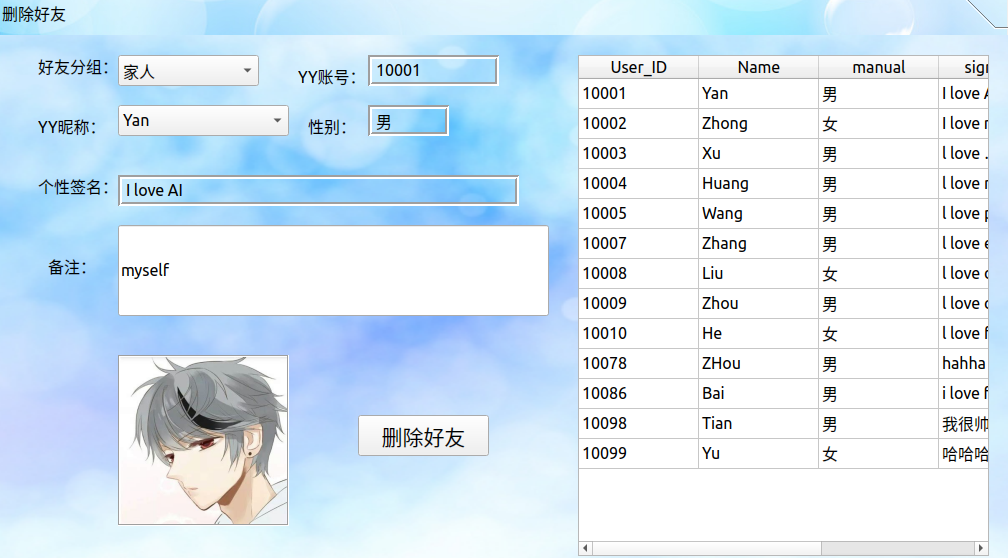
\includegraphics[width=0.7\textwidth]{7.png}
	\caption{\centering  “删除好友”页面效果图}
\end{figure}

\begin{table}[H]
	\renewcommand{\arraystretch}{1.0}
	\centering
	\caption{\centering “删除好友”页界面各控件属性设置}
	\begin{tabular}{lll}
		\toprule[1.5pt]
		名称                   & 类型          & 属性设置                                                                                                                                                                  \\
		\midrule[1pt]
preGroupComboBox     & QComboBox   & 默认                                                                                                                                                                    \\
preIDLineEdit        & QLineEdit   & 默认                                                                                                                                                                    \\
preNameLineEdit      & QLineEdit   & 默认                                                                                                                                                                    \\
premanualLineEdit    & QLineEdit   & 默认                                                                                                                                                                    \\
preSignatureLineEDit & QLineEdit   & 默认                                                                                                                                                                    \\
preReferenceLineEdit & QLineEdit   & 默认                                                                                                                                                                    \\
prePictureLabel      & QLabel      & \makecell[l]{frameshape:Box\\ frameShadow:Sunken\\text:空\\scaledContents:勾选      }                                                                                                       \\
DeletePushButton     & QPushButton & text:删除好友                                                                                                                                                             \\
FriendsTableView\_2  & QTableView  & \makecell[l]{horizontalHeaderVisibe:勾选\\ horizontalHeaderDefaultSectionSize:120\\ horizontalHeaderMinimumSectionSize:25\\ horizionHeaderStretchLastSection:勾选\\ verticalHeaderVisible:取消勾选}
		\\
		\bottomrule[1.5pt]
	\end{tabular}
\end{table}


\subsubsection{"好友信息"页}

“好友信息”页界面设计效果如下图所示,界面各控件属性设置见表

\begin{figure}[H]
	\centering
	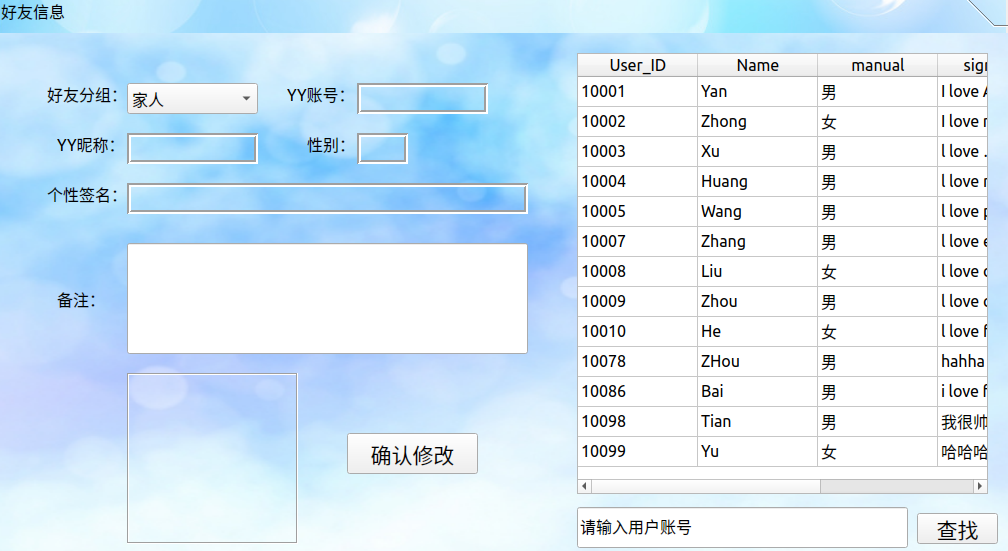
\includegraphics[width=0.6\textwidth]{8.png}
	\caption{\centering  “好友信息”页面效果图}
\end{figure}

\begin{table}[H]
	\renewcommand{\arraystretch}{1.0}
	\centering
	\caption{\centering “好友信息”页界面各控件属性设置}
	\begin{tabular}{lll}
		\toprule[1.5pt]
		名称                   & 类型          & 属性设置                                                                                                                                                                  \\
		\midrule[1pt]
fixedGroupComboBox         & QComboBox   & 默认                                                                                                                                                                    \\
fixedIDLineEdit            & QLineEdit   & 默认                                                                                                                                                                    \\
fixedNameLineEdit          & QLineEdit   & 默认                                                                                                                                                                    \\
fixedmanualLineEdit        & QLineEdit   & 默认                                                                                                                                                                    \\
fixedSignatureLineEDit     & QLineEdit   & 默认                                                                                                                                                                    \\
changableReferenceLineEdit & QLineEdit   & 默认                                                                                                                                                                    \\
SearchLineEdit             & QLineEdit   & text:请输入用户账号                                                                                                                                                          \\
fixedPictureLabel          & QLabel      & \makecell[l]{frameshape:Box\\ frameShadow:Sunken\\ text:空\\ scaledContents:勾选}                                                                                                            \\
ChangePushButton           & QPushButton & text:确认修改                                                                                                                                                             \\
SearchPushButton           & QPushButton & text:查找                                                                                                                                                               \\
FriendsTableView\_3        & QTableView  & \makecell[l]{horizontalHeaderVisibe:勾选\\ horizontalHeaderDefaultSectionSize:120\\ horizontalHeaderMinimumSectionSize:25\\ horizionHeaderStretchLastSection:勾选\\ verticalHeaderVisible:取消勾选}
		\\
		\bottomrule[1.5pt]
	\end{tabular}
\end{table}

\subsubsection{登录窗口}

登录窗口可以像程序主窗体一样在可视化设计器中进行设计,最终效果如下图所示,各控件属性设置见表

\begin{figure}[H]
	\centering
	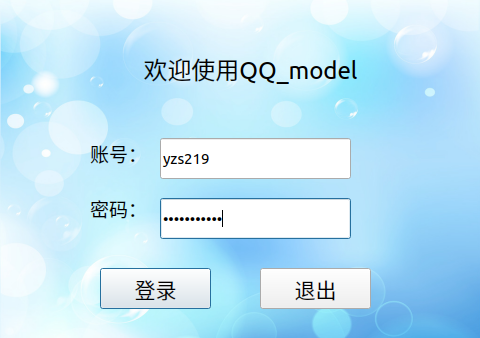
\includegraphics[width=0.5\textwidth]{9.png}
	\caption{\centering  登录窗口页面效果图}
\end{figure}

\begin{table}[H]
	\renewcommand{\arraystretch}{1.0}
	\centering
	\caption{\centering 登录窗口页界面各控件属性设置}
	\begin{tabular}{lll}
		\toprule[1.5pt]
		名称                   & 类型          & 属性设置                                                                                                                                                                  \\
		\midrule[1pt]
adminLineEdit   & QComboBox   & 默认                \\
pwdLineEdit     & QLineEdit   & echoMode:Password \\
loginPushButton & QPushButton & text:登录           \\
exitPushButton  & QPushButton & text:退出          \\
		\bottomrule[1.5pt]
	\end{tabular}
\end{table}

\subsection{MD5加密算法设计说明}

MD5以512位分组来处理输入的信息,且每一分组又被划分为16个32位子分组,经过了一系列的处理后,算法的输出由四个32位分组组成,将这四个32位分组级联后将生成一个128位散列值。

在MD5算法中,首先需要对信息进行填充,使其字节长度对512求余数的结果等于448。因此,信息的字节长度被扩展至N*512+448,即N*64+56个字节,N为一个正整数。填充的方法如下,在信息的后面填充一个1和无数个0,直到满足上面的条件时才停止用0对信息的填充。然后再在这个结果后面附加一个以64位二进制表示的填充前的信息长度。经过这两步的处理,现在的信息字节长度=N*512+448+64=(N+1)*512,即长度恰好是512的整数倍数。这样做的原因是为满足后面处理中对信息长度的要求。MD5中有四个32位被称作链接变量的整数参数,他们分别为:A=0x01234567,B=0x89abcdef,C=0xfedcba98,D=0x76543210。当设置好这四个链接变量后,就开始进入算法的四轮循环运算,循环的次数是信息中512位信息分组的数目。

将上面四个链接变量复制到另外四个变量中:A到a,B到b,C到c,D到d。主循环有四轮(MD4只有三轮),每轮循环都很相似。第一轮进行16次操作。每次操作对a、b、c和d中的其中三个作一次非线性函数运算,然后将所得结果加上第四个变量(文本中的一个子分组和一个常数)。

再将所得结果向右环移一个不定的数,并加上a、b、c或d中之一。最后用该结果取代a、b、c或d中之一。以一下是每次操作中用到的四个非线性函数(每轮一个)。

$$F(X,Y,Z)=(X\wedge Y)\vee ((\sim X)\wedge Z)$$
$$G(X,Y,Z)=(X\wedge Z)\vee (Y\wedge(\sim Z))$$
$$H(X,Y,Z)=X?Y?Z$$
$$\Gamma(X,Y,Z)=Y? (X\vee(\sim Z))$$

其中,$ ? $是异或,$\wedge $是与,$ \vee $是或,$ \sim $是反符号。

如果X、Y和Z的对应位是独立和均匀的,那么结果的每一位也应是独立和均匀的。F是一个逐位运算的函数。即,如果X,那么Y,否则Z。函数H是逐位奇偶操作符。所有这些完成之后,将A,B,C,D分别加上a,b,c,d。然后用下一分组数据继续运行算法,最后的输出是A,B,C和D的级联。最后得到的A,B,C,D就是输出结果,A是低位,D为高位,DCBA组成128位输出结果。

具体实现编码如下:

\begin{lstlisting}[language=c++]
QString LoginDialog::strToMd5(QString str)
{
	QString strMd5;
	QByteArray qba;
	qba=QCryptographicHash::hash(str.toLatin1(),QCryptographicHash::Md5);//调用QCryptographicHash类中生成密码散列的方法,生成二进制或文本数据的加密散列值
	strMd5.append(qba.toHex());
	return strMd5;
}	
\end{lstlisting}

\section{软件详细设计与编码}

\subsection{用户登录系统程序设计}

登录功能实现在logindialog.h头文件和logindialog.cpp源文件中,首先在logindialog.h中声明变量和方法,完整代码如下:

\begin{lstlisting}[language=c++]
#ifndef LOGINDIALOG_H
#define LOGINDIALOG_H

#include <QDialog>
#include <QSqlQuery>  //查询MYSQL的库
#include <QMessageBox> //弹窗信息提示库
#include <QCryptographicHash>  //包含MD5算法库
namespace Ui 
{
	class LoginDialog;
}
class LoginDialog : public QDialog
{
	Q_OBJECT
	public:
	explicit LoginDialog(QWidget *parent = 0);
	~LoginDialog();
	QString strToMd5(QString str);
	private slots:
	void on_loginPushButton_clicked();  //登录按钮单击事件槽
	void on_exitPushButton_clicked();   //退出按钮单击事件槽
	private:
	Ui::LoginDialog *ui;
};

#endif // LOGINDIALOG_H
然后,在logindialog.cpp源文件中实现登录验证功能,完整代码如下:
#include "logindialog.h"
#include "ui_logindialog.h"
LoginDialog::LoginDialog(QWidget *parent) :
QDialog(parent),
ui(new Ui::LoginDialog)
{
	ui->setupUi(this);
	setFixedSize(481,341);  //登录框固定大小
	ui->pwdLineEdit->setFocus();  //口令框置于焦点位置
}
LoginDialog::~LoginDialog()
{
	delete ui;
}
void LoginDialog::on_loginPushButton_clicked()
{
	if (!ui->pwdLineEdit->text().isEmpty())  //判断输入是否为空
	{
		QSqlQuery query;
		query.exec("select PassWord from Member where MemberID='"+  ui->adminLineEdit->text() + "'");  //从数据库查询口令密码
		query.next();
		QString pwdMd5=strToMd5(ui->pwdLineEdit->text());//将用户输入的口令字符串转为MD5加密串
		if (query.value(0).toString() == pwdMd5)  
		{
			QDialog::accept();  //验证通过
		}
		else
		{
			QMessageBox::warning(this,tr("密码错误"),tr("请重新输入密码!"),QMessageBox::Ok);
			ui->pwdLineEdit->clear();
			ui->pwdLineEdit->setFocus();
		}
	}
	else
	{
		ui->pwdLineEdit->setFocus();
	}
}
void LoginDialog::on_exitPushButton_clicked()
{
	QDialog::reject();//退出登录界面
}
QString LoginDialog::strToMd5(QString str)  //MD5加密方法
{
	QString strMd5;
	QByteArray qba;
	qba=QCryptographicHash::hash(str.toLatin1(),QCryptographicHash::Md5);
	strMd5.append(qba.toHex());
	return strMd5;
}
\end{lstlisting}

\subsection{主体程序框架}

\begin{enumerate}[itemsep=0.01pt]
	\item[(1)]main.cpp

它是整个系统的主启动文件,代码如下:

\begin{lstlisting}[language=c++]
#include "mainwindow.h"
#include "logindialog.h"
#include <QProcess>  //Qt进程模块
#include <QApplication>

int main(int argc, char *argv[])
{
	QApplication a(argc, argv);
	if (!createMysqlConn()) //判断数据库连接情况
	{
		QProcess process;
		process.start("/usr/sbin/mysqld.exe");
		if (!createMysqlConn()) return 1;
	}
	LoginDialog logindlg; //登录对话框
	if (logindlg.exec()==QDialog::Accepted)
	{
		MainWindow w;
		w.show();   //启动主窗体
		return a.exec();
	}
	else
	{
		return 0;
	}
}

\end{lstlisting}

\item[(2)]mainwindow.h

它是程序头文件,包含程序中用到的各个全局变量的定义、方法声明,完整代码如下:

\begin{lstlisting}[language=c++]
#ifndef MAINWINDOW_H
#define MAINWINDOW_H
#include <QMainWindow>
#include <QMessageBox>
#include <QFileDialog>
#include <QBuffer>
#include "opencv2/opencv.hpp"  //Opencv文件包含
#include <QSqlDatabase>        //MySQL数据库类
#include <QSqlTableModel>      //MySQL表模型类
#include <QSqlQuery>           //MySQL查询库类
#include <QTime>
#include <QPixmap>             //图像处理类库
using namespace cv;  //opencv命名空间
namespace Ui { class MainWindow; }
class MainWindow : public QMainWindow
{
	Q_OBJECT
	public:
	explicit MainWindow(QWidget *parent = 0);
	~MainWindow();
	void initMainWindow();  //界面初始化方法
	void onTableSelectChange(int row);  //用户在好友列表网格选取好友时进行好友信息表单更新
	void showFriendPhoto();  //显示好友头像
	void loadPreFriends();  //“删除好友”页:对应分组加载好友列表
	void onPreNameComboBoxChange();  //“删除好友”页:改选好友时联动显示好友信息
	private slots:
	void on_FriendsTableView_3_clicked(const QModelIndex &index); //“好友信息”页:联动显示好友信息
	void on_preGroupComboBox_currentIndexChanged(int index); //“删除好友”页:根据类别对应加载对应好友列表
	void on_preNameComboBox_currentIndexChanged(int index);//“删除好友”页:选择好友时联动显示好友信息
	void on_DeletePushButton_clicked();  //删除好友操作
	void on_newUploadPushButton_clicked();  //上传头像
	void on_NewPutinPushButton_clicked(); //添加好友
	void on_ChangePushButton_clicked();//修改备注
	void on_SearchPushButton_clicked();//搜索好友
	private:
	Ui::MainWindow *ui;
	QImage myPicImg;  //保存好友头像
	QSqlTableModel *friends_model;  //访问数据库好友信息视图的模型
};
static bool createMysqlConn()  //访问MySQL数据库的静态方法
{
	QSqlDatabase sqldb=QSqlDatabase::addDatabase("QMYSQL");
	sqldb.setHostName("127.0.0.1");  //主机名
	sqldb.setDatabaseName("friendsList");  //数据库名称
	sqldb.setPort(3306); //接口名
	sqldb.setUserName("root"); //用户名
	sqldb.setPassword("20020619");//登录密码
	if (!sqldb.open())
	{
		QMessageBox::critical(0,QObject::tr("后台数据库连接失败"),"无法创建连接!请检查故障后重新连接!",QMessageBox::Cancel);
		return false;
	}
	return true;
}
#endif // MAINWINDOW_H

\end{lstlisting}

\item[(3)]mainwindow.cpp

它是本程序的主体源文件,其中包含各方法功能的具体实现代码,完整代码见附录1.

\end{enumerate}

\section{总结分析与感悟}

\subsection{主要完成工作说明}
本次实践,我主要负责了模拟QQ的第三版开发工作,运用SQL作为后台依赖,基于QT Creator进行软件开发,独立设立了软件UI,运用C++编写了相关功能方法代码,实现了相关接口连接,完成了软件大体设计。

\subsection{软件缺陷及改进}
\begin{itemize}[itemsep=0.01pt]
\item	鼠标右键的触发事件由于时间原因尚未完成总体设计,MySQL中Group表还可以进行优化以实现分组的添加删除等功能;好友查找功能对于输入首字母弹出对于好友列表尚未实现,可再利用一个ComBoBox完成此项设计。
\item	目前只是单用户管理员身份运行,未来可增加用户注册与服务器运行功能,实现多用户交互式平台与多用户聊天室窗口。
\item	UI界面不够集成化,可将好友列表利用Tree View进行展示,显得更加有层次性;其次,可单独将Table View置于新页面,单独作为好友信息展示区,则界面看起来更为轻量化。
\item	由于时间原因未来得及设计好友交互页面,可再设计一个UI界面作为聊天框并通过socket网络编程运用TCP协议进行信息传输实现聊天交互,同时在数据库中设计新表以存储聊天信息与时间节点。
\end{itemize}

\subsection{软件设计未来规划}
\begin{itemize}[itemsep=0.01pt]
\item	完善软件基础功能,优化UI界面
\item	实现多用户服务器交互式聊天平台,具备独立聊天窗口与群聊界面
\item	实现网络编程,用户间可通过TCP网络协议实现信息传输
\item	实现聊天信息存储,增加历史聊天记录查看及查找功能
\end{itemize}

\newpage
\begin{center}
	\Large{\textbf{\heiti 附录}}
\end{center}

\appendix
% \renewcommand{\appendixname}{Appendix~\Alph{section}}
\section{附录 1 -- mainwindow.cpp 程序代码 }

\begin{lstlisting}[language=c++]

#include "mainwindow.h"
#include "ui_mainwindow.h"

MainWindow::MainWindow(QWidget *parent)
: QMainWindow(parent)
, ui(new Ui::MainWindow)
{
	/*setwindowicon*/
	//setWindowIcon(QIcon(QStringLiteral(":/background/mainlogo")));
	ui->setupUi(this);
	initMainWindow(); //执行初始化方法
}
MainWindow::~MainWindow()
{
	delete ui;
}

void MainWindow::initMainWindow()  //对系统主窗体进行初始化
{
	//Qt::WindowFlags flags = this->windowFlags();
	//this->setWindowFlags(flags|Qt::WindowStaysOnTopHint);
	ui->stackedWidget->setCurrentIndex(1);  //置于好友管理页面
	ui->Friend_Operation->setCurrentIndex(0);     //“添加好友”页置于前面
	QSqlQueryModel *GroupModel = new QSqlQueryModel(this);  //好友类别模型数据
	GroupModel->setQuery("select Group_Name from `Group`");
	//QStringList strings;
	//QSqlQuery query("SELECT Group_Name FROM Group");
	//while (query.next()) {
		//        QString group_name = query.value(0).toString();
		//      strings.append(group_name);
		//}
	//ui->newGroupComboBox->addItems(strings);
	friends_model=new QSqlTableModel(this);  //好友信息视图
	friends_model->setTable("friends_inf");
	friends_model->select();
	ui->FriendsTableView->setModel(friends_model);   //初始化好友列表
	ui->FriendsTableView_2->setModel(friends_model);
	ui->FriendsTableView_3->setModel(friends_model);
	ui->newGroupComboBox->setModel(GroupModel);  //初始化下拉框
	ui->preGroupComboBox->setModel(GroupModel);
	ui->fixedGroupComboBox->setModel(GroupModel);
	loadPreFriends();
}
void MainWindow::onTableSelectChange(int row)  //“好友信息”页:用户选择信息时进行表单更新
{
	int r=1;
	if (row!=0) r=ui->FriendsTableView_3->currentIndex().row();
	QModelIndex index;
	index=friends_model->index(r,0);  //ID
	ui->fixedIDLabel->setText(friends_model->data(index).toString());
	index=friends_model->index(r,1);  //name
	ui->fixedNameLabel->setText(friends_model->data(index).toString());
	index=friends_model->index(r,2);  //manual
	ui->fixedmanualLabel->setText(friends_model->data(index).toString());
	index=friends_model->index(r,3);  //signature
	ui->fixedsignatureLabel->setText(friends_model->data(index).toString());
	index=friends_model->index(r,4);  //reference
	ui->changableReferenceLineEdit->setText(friends_model->data(index).toString());
	showFriendPhoto();
	QSqlQuery query;
	query.exec(QString("select Group_Name from `Group` where Group_ID=(select Group_ID from FriendsList where Name='%1')").arg(ui->fixedNameLabel->text()));
	query.next();
	ui->fixedGroupComboBox->setCurrentText(query.value(0).toString());  //实现分组信息联动
}
void MainWindow::showFriendPhoto()  //显示头像
{
	QPixmap photo;
	QModelIndex index;
	QSqlQueryModel *pictureModel =new QSqlQueryModel(this);
	QString name=ui->fixedNameLabel->text();
	pictureModel->setQuery("select Picture from FriendsList where Name='"+name+"'");
	index=pictureModel->index(0,0);
	photo.loadFromData(pictureModel->data(index).toByteArray(),"JPG");
	ui->fixedpictureLabel->setPixmap(photo);
}
void MainWindow::loadPreFriends()  //“删除好友”页:对应分组加载好友列表
{
	QSqlQueryModel *friends_name_model=new QSqlQueryModel(this);  //好友名称模型数据
	friends_name_model->setQuery(QString("select Name from FriendsList where Group_ID=(select Group_ID from `Group` where Group_Name='%1')")\
	.arg(ui->preGroupComboBox->currentText()));//加载好友列表
	ui->preNameComboBox->setModel(friends_name_model);
	onPreNameComboBoxChange();
}
void MainWindow::onPreNameComboBoxChange()  //“删除好友”页:改选好友时联动显示好友信息
{
	QSqlQueryModel *PreFriendsModel=new QSqlQueryModel(this);
	QString name=ui->preNameComboBox->currentText();
	PreFriendsModel->setQuery("select User_ID,manual,signature,reference,Picture from FriendsList where Name='"+name+"'");
	QModelIndex index;
	index=PreFriendsModel->index(0,0);  //账号
	ui->preIDLabel->setText(PreFriendsModel->data(index).toString());
	index=PreFriendsModel->index(0,1);  //性别
	ui->preManualLabel->setText(PreFriendsModel->data(index).toString());
	index=PreFriendsModel->index(0,2);  //个性签名
	ui->preSignatureLabel->setText(PreFriendsModel->data(index).toString());
	index=PreFriendsModel->index(0,3);  //备注
	ui->preReferenceLineEdit->setText(PreFriendsModel->data(index).toString());
	//获取头像
	QPixmap photo;
	index=PreFriendsModel->index(0,4);
	photo.loadFromData(PreFriendsModel->data(index).toByteArray(),"JPG");
	ui->prePictureLabel->setPixmap(photo);
}
void MainWindow::on_FriendsTableView_3_clicked(const QModelIndex &index)  //“好友信息”页:联动显示好友信息
{
	onTableSelectChange(1);
}
void MainWindow::on_preGroupComboBox_currentIndexChanged(int index)   //“删除好友”页:根据类别对应加载对应好友列表
{
	loadPreFriends();
}
void MainWindow::on_preNameComboBox_currentIndexChanged(int index)  //“删除好友”页:选择好友时联动显示好友信息
{
	onPreNameComboBoxChange();
}
void MainWindow::on_DeletePushButton_clicked()  //“删除好友”页:删除好友操作
{
	QSqlQuery query;
	query.exec(QString("delete from FriendsList where Name='%1'").arg(ui->preNameComboBox->currentText()));//删除好友记录
	//刷新界面
	ui->preManualLabel->setText("");
	ui->preSignatureLabel->setText("");
	ui->preIDLabel->setText("");
	ui->preReferenceLineEdit->setText("");
	ui->prePictureLabel->clear();
	friends_model->setTable("friends_inf");
	friends_model->select();
	//刷新数据网格
	ui->FriendsTableView->setModel(friends_model);
	ui->FriendsTableView_2->setModel(friends_model);
	ui->FriendsTableView_3->setModel(friends_model);
}
void MainWindow::on_newUploadPushButton_clicked()  //上传头像
{
	QString picturename=QFileDialog::getOpenFileName(this,"选择头像",".","Image File(*.png *.jpg *.jpeg *.bmp)");
	if (picturename.isEmpty()) return;
	myPicImg.load(picturename);
	ui->NewPictureLabel->setPixmap(QPixmap::fromImage(myPicImg));
}
void MainWindow::on_NewPutinPushButton_clicked() //添加好友
{
	QSqlQuery query;
	query.exec(QString("select Group_ID from `Group` where Group_Name='%1'").arg(ui->newGroupComboBox->currentText()));
	query.next();
	int Group_ID=query.value(0).toInt();
	QString name =ui->newNameLineEdit->text();
	int User_ID=ui->newIDLineEdit->text().toInt();
	QString maunal=ui->newmanualLineEdit->text();
	QString signature=ui->newSignatureLineEdit->text();
	QString reference=ui->newRefenrenceLineEdit->text();
	query.exec(QString("insert into FriendsList(User_ID,Group_ID,Name,manual,signature,reference,Picture)values(%1,%2,'%3','%4','%5','%6',NULL)")\
	.arg(User_ID).arg(Group_ID).arg(name).arg(maunal).arg(signature).arg(reference));//添加好友信息
	//插入照片
	QByteArray picdata;
	QBuffer buffer(&picdata);
	buffer.open(QIODevice::WriteOnly);
	myPicImg.save(&buffer,"JPG");
	QVariant var(picdata);
	QString sqlstr="update FriendsList set Picture=? where Name='"+name+"'";
	query.prepare(sqlstr);
	query.addBindValue(var);
	if (!query.exec())
	{
		QMessageBox::information(0,QObject::tr("提示"),"添加失败");
	}
	else
	{
		QMessageBox::information(0,QObject::tr("提示"),"添加成功!");
	}
	ui->newIDLineEdit->setText("");
	ui->newNameLineEdit->setText("");
	ui->newmanualLineEdit->setText("");
	ui->newSignatureLineEdit->setText("");
	ui->newRefenrenceLineEdit->setText("");
	ui->NewPictureLabel->clear();
	friends_model->setTable("friends_inf");   //刷新网格信息
	friends_model->select();
	ui->FriendsTableView->setModel(friends_model);
	ui->FriendsTableView_2->setModel(friends_model);
	ui->FriendsTableView_3->setModel(friends_model);
}
void MainWindow::on_ChangePushButton_clicked()  //“好友信息”页:修改好友信息
{
	QSqlQuery query;
	QString new_reference=ui->changableReferenceLineEdit->text();
	query.exec(QString("update FriendsList set reference='%1' where Name='%2'").arg(new_reference).arg(ui->fixedNameLabel->text()));
	if (!query.exec())
	{
		QMessageBox::information(0,QObject::tr("提示"),"修改失败");
	}
	else
	{
		QMessageBox::information(0,QObject::tr("提示"),"修改成功!");
	}
	friends_model->setTable("friends_inf");   //刷新网格信息
	friends_model->select();
	ui->FriendsTableView->setModel(friends_model);
	ui->FriendsTableView_2->setModel(friends_model);
	ui->FriendsTableView_3->setModel(friends_model);
}
void MainWindow::on_SearchPushButton_clicked()  //搜索好友
{
	QSqlQuery query;
	query.exec(QString("select User_ID,Group_ID,Name,manual,signature,reference,Picture from FriendsList where User_ID='%1'").\
	arg(ui->SearchLineEdit->text().toInt()));
	if (query.exec())
	{
		query.next();
		ui->fixedIDLabel->setText(query.value(0).toString());
		ui->fixedNameLabel->setText(query.value(2).toString());
		ui->fixedmanualLabel->setText(query.value(3).toString());
		ui->fixedsignatureLabel->setText(query.value(4).toString());
		ui->changableReferenceLineEdit->setText(query.value(5).toString());
		showFriendPhoto();
		query.exec(QString("select Group_Name from `Group` where Group_ID=(select Group_ID from FriendsList where Name='%1')").\
		arg(ui->fixedNameLabel->text()));
		query.next();
		ui->fixedGroupComboBox->setCurrentText(query.value(0).toString());
	}
	else
	{
		QMessageBox::information(0,QObject::tr("提示"),"未检测到此好友");
	}
}
\end{lstlisting}

\addcontentsline{toc}{section}{参考文献}%将“参考文献加入目录中”
\begin{thebibliography}{99}
	\bibitem{1}陆文周.Qt5开发及实例(第4版)[M].电子工业出版社:北京,2019:403-434.
	\bibitem{2}汤研.基于TCP的简易聊天室设计与实现[J].电脑编程技巧与维护,2020(12):27-29.
\end{thebibliography}

\end{document}
